% $Id: template.tex 11 2007-04-03 22:25:53Z jpeltier $


\documentclass{vgtc}                          % final (conference style)
%\documentclass[review]{vgtc}                 % review
%\documentclass[widereview]{vgtc}             % wide-spaced review
%\documentclass[preprint]{vgtc}               % preprint
%\documentclass[electronic]{vgtc}             % electronic version

\makeatletter
\let\@citex\asme@citex % restore
\makeatother

%% Uncomment one of the lines above depending on where your paper is
%% in the conference process. ``review'' and ``widereview'' are for review
%% submission, ``preprint'' is for pre-publication, and the final version
%% doesn't use a specific qualifier. Further, ``electronic'' includes
%% hyperreferences for more convenient online viewing.

%% Please use one of the ``review'' options in combination with the
%% assigned online id (see below) ONLY if your paper uses a double blind
%% review process. Some conferences, like IEEE Vis and InfoVis, have NOT
%% in the past.

%% Figures should be in CMYK or Grey scale format, otherwise, colour 
%% shifting may occur during the printing process.

%% These few lines make a distinction between latex and pdflatex calls and they
%% bring in essential packages for graphics and font handling.
%% Note that due to the \DeclareGraphicsExtensions{} call it is no longer necessary
%% to provide the the path and extension of a graphics file:
%% \includegraphics{diamondrule} is completely sufficient.
%%
\ifpdf%                                % if we use pdflatex
  \pdfoutput=1\relax                   % create PDFs from pdfLaTeX
  \pdfcompresslevel=9                  % PDF Compression
  \pdfoptionpdfminorversion=7          % create PDF 1.7
  \ExecuteOptions{pdftex}
  \usepackage{graphicx}                % allow us to embed graphics files	
  \DeclareGraphicsExtensions{.pdf,.png,.jpg,.jpeg} % for pdflatex we expect .pdf, .png, or .jpg files
\else%                                 % else we use pure latex
  \ExecuteOptions{dvips}
  \usepackage{graphicx}                % allow us to embed graphics files
  \DeclareGraphicsExtensions{.eps}     % for pure latex we expect eps files
\fi%

%% it is recomended to use ``\autoref{sec:bla}'' instead of ``Fig.~\ref{sec:bla}''
\graphicspath{size_and_scatterplots_files/figure-latex} % where to search for the images

\usepackage{microtype}                 % use micro-typography (slightly more compact, better to read)
\PassOptionsToPackage{warn}{textcomp}  % to address font issues with \textrightarrow
\usepackage{textcomp}                  % use better special symbols
\usepackage{mathptmx}                  % use matching math font
\usepackage{times}
\usepackage[T1]{fontenc}               % we use Times as the main font
\renewcommand*\ttdefault{txtt}         % a nicer typewriter font
\usepackage{cite}                      % needed to automatically sort the references
\usepackage{tabu}                      % only used for the table example
\usepackage{booktabs}                  % only used for the table example
%% We encourage the use of mathptmx for consistent usage of times font
%% throughout the proceedings. However, if you encounter conflicts
%% with other math-related packages, you may want to disable it.


%% If you are submitting a paper to a conference for review with a double
%% blind reviewing process, please replace the value ``0'' below with your
%% OnlineID. Otherwise, you may safely leave it at ``0''.
\onlineid{0}

%% declare the category of your paper, only shown in review mode
\vgtccategory{Research}

%% allow for this line if you want the electronic option to work properly
\vgtcinsertpkg

%% In preprint mode you may define your own headline. If not, the default IEEE copyright message will appear in preprint mode.
%\preprinttext{To appear in an IEEE VGTC sponsored conference.}

%% This adds a link to the version of the paper on IEEEXplore
%% Uncomment this line when you produce a preprint version of the article 
%% after the article receives a DOI for the paper from IEEE
%\ieeedoi{xx.xxxx/TVCG.201x.xxxxxxx}


%% Paper title.

\title{A Novel Technique to Facilitate More Accurate Correlation Perception in Scatterplots}

%% This is how authors are specified in the conference style

%% Author and Affiliation (single author).
%%\author{Roy G. Biv\thanks{e-mail: roy.g.biv@aol.com}}
%%\affiliation{\scriptsize Allied Widgets Research}

%% Author and Affiliation (multiple authors with single affiliations).
%%\author{Roy G. Biv\thanks{e-mail: roy.g.biv@aol.com} %
%%\and Ed Grimley\thanks{e-mail:ed.grimley@aol.com} %
%%\and Martha Stewart\thanks{e-mail:martha.stewart@marthastewart.com}}
%%\affiliation{\scriptsize Martha Stewart Enterprises \\ Microsoft Research}

%% Author and Affiliation (multiple authors with multiple affiliations)
\author{Gabriel Strain\thanks{\href{mailto:Gabriel.Strain@manchester.ac.uk}{\nolinkurl{Gabriel.Strain@manchester.ac.uk}}} %
\and Andrew J. Stewart\thanks{\href{mailto:Andrew.J.Stewart@manchester.ac.uk}{\nolinkurl{Andrew.J.Stewart@manchester.ac.uk}}} %
\and Paul Warren\thanks{\href{mailto:Paul.Warren@manchester.ac.uk}{\nolinkurl{Paul.Warren@manchester.ac.uk}}} %
\and Caroline Jay\thanks{\href{mailto:Caroline.Jay@manchester.ac.uk}{\nolinkurl{Caroline.Jay@manchester.ac.uk}}}} %
 \affiliation{\scriptsize The University of Manchester}


%% Abstract section.
\abstract{Viewers consistently underestimate correlation in positively correlated scatterplots.
We use a novel data point size manipulation to correct for this bias. In a high-powered and
fully reproducible study, we demonstrate that decreasing the size of a point on a scatterplot
as a function of its distance from the regression line is able to correct for a systematic
perceptual bias long present in the literature. We suggest the implementation of our technique
when designing scatterplots that aim to communicate positive correlations.}

%% ACM Computing Classification System (CCS). 
%% See <http://www.acm.org/about/class> for details.
%% We recommend the 2012 system <http://www.acm.org/about/class/class/2012>
%% For the 2012 system use the ``\CCScatTwelve'' which command takes four arguments.
%% The 1998 system <http://www.acm.org/about/class/class/2012> is still possible
%% For the 1998 system use the ``\CCScat'' which command takes four arguments.
%% In both cases the last two arguments (1998) or last three (2012) can be empty.

\CCScatlist{
  \CCScatTwelve{Human-centered computing}{Visu\-al\-iza\-tion}{Empirical studies in visualization};
  \CCScatTwelve{Human-centered computing}{Human computer interaction (HCI)}{Empirical studies in HCI}
}

%\CCScatlist{
  %\CCScat{H.5.2}{User Interfaces}{User Interfaces}{Graphical user interfaces (GUI)}{};
  %\CCScat{H.5.m}{Information Interfaces and Presentation}{Miscellaneous}{}{}
%}

%% Copyright space is enabled by default as required by guidelines.
%% It is disabled by the 'review' option or via the following command:
% \nocopyrightspace

%%%%%%%%%%%%%%%%%%%%%%%%%%%%%%%%%%%%%%%%%%%%%%%%%%%%%%%%%%%%%%%%
%%%%%%%%%%%%%%%%%%%%%% START OF THE PAPER %%%%%%%%%%%%%%%%%%%%%%
%%%%%%%%%%%%%%%%%%%%%%%%%%%%%%%%%%%%%%%%%%%%%%%%%%%%%%%%%%%%%%%%%

\begin{document}

%% The ``\maketitle'' command must be the first command after the
%% ``\begin{document}'' command. It prepares and prints the title block.

%% the only exception to this rule is the \firstsection command
\firstsection{}

\maketitle

\hypertarget{introduction}{%
\section{Introduction}\label{introduction}}

Scatterplots, utilized in scientific communication for a variety of tasks,
are some of the most widely used and studied data visualizations. Viewers
interpret them in similar ways \cite{kay_heer_2015}, and they are simple
enough to be easily studied while providing important insights into visualization
design, human-computer interaction, and perception. In a previous study \cite{strain_2023},
we showed that a novel point contrast manipulation, in which the contrast of a certain
scatterplot point was reduced as the size of that point's residual increased, could be
used to partially correct for a systematic correlation underestimation bias present in the
literature \cite{strahan_1978, bobko_1979, cleveland_1982, lane_1985, lauer_1989, 
collyer_1990, meyer_1992}. We suggested that this was due to a narrowing of the width
of the perceived probability distribution of a plot brought
about by the lower contrast (and therefore lower point-salience and higher spatial uncertainty)
in those outer areas. In that study we tested linear, non-linear, and non-linear inverted functions relating
point contrast to residual size, finding that the non-linear function produced
the most accurate estimates of correlation, and that the non-linear inverted produced
the least accurate. In the present study we use the same equations to manipulate
point size.

\hypertarget{scatterplots-and-correlation}{%
\subsection{Scatterplots and Correlation}\label{scatterplots-and-correlation}}

Scatterplots have been widely studied, especially as mediums for the communication
of correlation (see \cite{strain_2023} for a full review of the history of this work).
Previous literature has found evidence for a pronounced underestimation in judgements
of correlation in positively correlated scatterplots, especially between 0.2 \textless{} \emph{r} \textless{} 0.6. This
has held true for both direct estimation \cite{meyer_1992, collyer_1990} and estimation
via bisection tasks \cite{rensink_2017}. In addition to work exploring how we
perceive the magnitude of correlation, in more recent years methods from psychophysics
have been employed to explore how we discriminate between different correlations
\cite{rensink_2014, rensink_2017}. As in our previous work,
we use the direct estimation paradigm owing to its simplicity and its suitability
to online experimentation. This renders the judgements we collect
comparative by nature, as we analyse the difference in correlation estimation performance
between data-identical scatterplots with different point size manipulations (see Figure \ref{fig:examples}).
Such work allows us to inform design guidelines and affords us insights into perception.
It is our duty as visualization designers to ensure that the
messages we are trying to communicate are being interpreted as accurately as possible
by viewers. To achieve this, we must understand human perception, apply that understanding
to design, and test those designs in rigorous empirical studies.

\hypertarget{point-size}{%
\subsection{Point Size}\label{point-size}}

While contrast adjustments have been used extensively to solve issues of overplotting and clutter
in scatterplots \cite{matejka_2015, bertini_2004}, there is no established use of
varying point size. Common sense dictates that scatterplots visualizing larger
datasets inherently require their points to be smaller to prevent obfuscation of the data,
but there is little testing of the impact of point size on correlation perception.
Studies have found invariance in the bias and variability of correlation
perception with regards to changing point sizes, but these have been low-powered
\cite{rensink_2012, rensink_2014}. From the wider literature there is evidence
that larger points are more salient \cite{healey_2012}, can bias judgements of
mean point position more strongly than point contrast can \cite{hong_2021}, and can
result in faster reaction times to peripherally presented stimuli \cite{grice_1983}.
In addition, smaller stimuli are associated with greater levels of spatial uncertainty
\cite{alais_2004}, and if this uncertainty is driving the reduction in bias we saw in our previous work \cite{strain_2023},
we would expect a similar effect when point size is used instead of point contrast.

\hypertarget{hypotheses}{%
\subsection{Hypotheses}\label{hypotheses}}

We hypothesized that correlation estimates would be most accurate when
viewers are presented with the non-linear size decay condition, and would be
least accurate when presented with the non-linear inverted size decay condition.
We therefore present a single experiment study in which we demonstrate that the use of
a non-linear size decay function relating to the residuals of points on scatterplots
can be employed to correct for a systematic underestimation of correlation by
viewers. We find no evidence for effects of graph literacy or training.
The effect we observe here is much stronger, both
with regards to effect size and in terms of the observed reduction in error, than that
observed in our previous study \cite{strain_2023}. We suggest that this
function can be used to facilitate more accurate correlation
perception in scatterplots, and provides exciting future avenues for the continuation
and refinement of these techniques. Ethical approval was granted by the University
of Manchester's Computer Science Departmental Panel (Ref: 2022-14660-24397).

\hypertarget{methodology}{%
\section{Methodology}\label{methodology}}

The experiment was conducted according to the principles of open and reproducible research.
All data and analysis code are available at \url{https://github.com/gjpstrain/size_and_scatterplots}.
This repository contains instructions for building a docker image to fully
reproduce the computational environment used, allowing for full replications
of stimulus generation, analyses, and the paper itself. Hypotheses and analysis plans were
pre-registered with the OSF (\url{https://osf.io/k4gd8}).

\hypertarget{participants}{%
\subsection{Participants}\label{participants}}

150 participants were recruited using the Prolific.co platform. Normal to
corrected-to-normal vision and English fluency were required for participation. As in our previous work
\cite{strain_2023}, and in accordance with previously published guidelines \cite{peer_2021},
participants were required to have completed at least 100 studies on Prolific, and were
required to have a Prolific score of at least 100, indicating acceptance on at least
100/101 previously completed studies. Participants who took part in any of our
previous studies on correlation perception in scatterplots
were prevented from participating, and participants were only
permitted to complete the experiment on a desktop or laptop computer.

Data were collected from 164 participants. 14 failed more than 2 out of 6 attention
checks, and, as per pre-registration stipulations, were rejected from the study. Data
from 150 participants was included in the analysis (48\% male, 50\% female, and 2\% non-binary). Mean age of participants was 29.6 (\emph{SD} = 8.5). Mean graph literacy score was 21.77
(\emph{SD} = 4.29) out of 30. The average time taken to complete
the experiment was 39 minutes (\emph{SD} = 14 minutes).

\hypertarget{stimuli}{%
\subsection{Stimuli}\label{stimuli}}

The data used to generated the scatterplots in the current study were identical to that
used previously \cite{strain_2023}. Scatterplots were generated based on 45 uniformly
distributed \emph{r} values between 0.2 and 0.99, as there is evidence from the literature
that little correlation is perceived below \emph{r} = 0.2 \cite{strahan_1978, bobko_1979, cleveland_1982}.
A total of 45 \emph{r} values were chosen so that we could build a more detailed picture
of people's perceptions of correlations than previous work using fewer values,
in addition to affording us a more objective method of comparing people's judgements
beyond semantic labels such as `weak' or `strong' correlation as response measures.
Previous work, including our own, used only positive \emph{r} values, and as we are building on this
here, we do the same. Scatterplot points were generated based on bivariate normal distributions with
standard deviations of 1 in each direction. Each scatterplot had a 1:1 aspect ratio,
was generated as a 1200 x 1200 pixel .png image, and was
scaled up or down according to the participant's monitor. See
\autoref{dot-pitch-and-crowdsourced-experiments} for a more detailed discussion of
precise point sizes and dot pitch in crowd-sourced experiments.

As in our previous study \cite{strain_2023} we used equation 1 to map residuals
to point sizes in three of our conditions. We additionally used a scaling factor
of 4 and a constant of 0.2 to achieve a minimum on-screen point size of 12 pixels,
which is consistent with the point size on a 1920 x 1080 monitor for both experiments
in our previous study \cite{strain_2023}. In our fourth condition, which we henceforth refer to as \emph{standard size},
point size was uniformly set to be consistent with the point size in our previous
studies. Scripts detailing scatterplot and mask generation can be found in the item
preparation folder in the repository linked above.

\begin{equation}
  point_{size} = 1 - b^{residual}
\end{equation}

\hypertarget{dot-pitch-and-crowdsourced-experiments}{%
\subsection{Dot Pitch and Crowdsourced Experiments}\label{dot-pitch-and-crowdsourced-experiments}}

In our previous study \cite{strain_2023} we had no way of obtaining dot pitch
or participant to monitor distance due to the online, crowdsourced nature of the
experiments. We have since adopted a method for obtaining the height of a
participant's monitor in inches \cite{screenscale}; participants are asked to hold up a standard size
credit/debit/ID card up to the monitor, and then to resize a corresponding image until
it matches the physical size of the card. These cards have a universal
standard size (ISO/IEC 7810 ID-1), which when combined with
the monitor resolution obtained from PsychoPy \cite{pierce_psychopy_2019}
and assuming a widescreen 16:9 aspect ratio,
allows us to infer dot pitch and therefore the physical size of the points in our
experiment. Mean dot pitch was 0.33mm (\(SD = 0.06\)),
corresponding to a physical size on the screen of 4.32mm
for the smallest points displayed. See \autoref{results} for analyses including dot pitch as a predictor.

\hypertarget{visual-threshold-testing}{%
\subsection{Visual Threshold Testing}\label{visual-threshold-testing}}

It is key that our manipulation does not remove data from the scatterplot,
thus, in order to test that all our points were visible across a range of viewing
contexts and on a range of apparatus, we included visual threshold testing prior
to the experimental items in the study. Participants were shown six scatterplots
and were asked to enter in a text box how many points
were being displayed. The points were the same size as the smallest points used
in the experimental materials. 5\% of
participants were correct on 5 out of 6 visual
threshold questions, while 95\% were correct
on 6 out of 6. It should be noted that those
participants scoring 5/6 did not answer incorrectly, rather they did not answer
at all for a particular question, which is suggestive of
a mis-click or an initial misunderstanding of the task. Regardless,
we consider these results to be indicative of a sufficient level of
point visibility.

\hypertarget{design}{%
\subsection{Design}\label{design}}

The experiment used a fully repeated measures, within-participants design, with each
participant seeing and responding to each of the 180 scatterplots in a randomized order.
There were four scatterplots for each of the 45 \emph{r} values corresponding to the
four levels of the size decay condition, examples of which can be see in Figure \ref{fig:examples}.
Everything needed to run the experiment, including code, materials, instructions, and scripts, is
hosted at \url{https://gitlab.pavlovia.org/Strain/exp_size_only}.

\begin{figure}
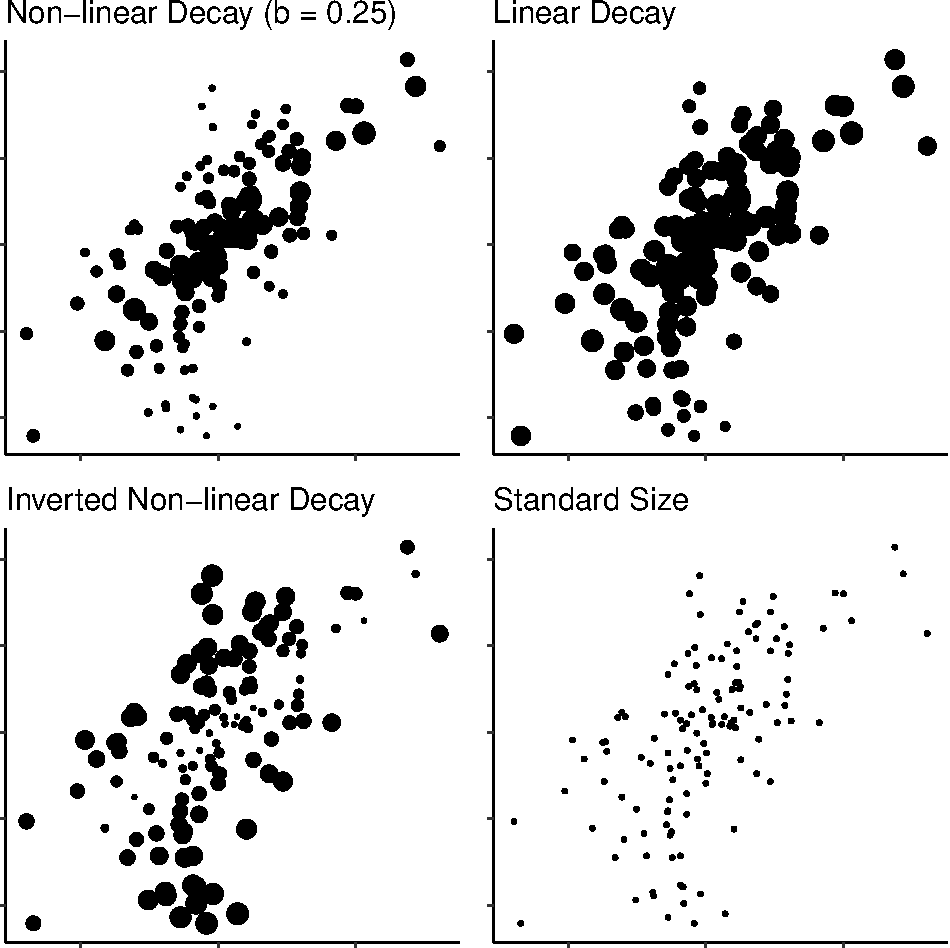
\includegraphics[width=1\linewidth]{size_and_scatterplots_files/figure-latex/examples-1} \caption{Four levels of the point size decay condition, demonstrated with an \textit{r} value of 0.6}\label{fig:examples}
\end{figure}

\hypertarget{procedure}{%
\subsection{Procedure}\label{procedure}}

Each participant was shown the participant information sheet and provided
consent through key presses in response to consent statements. They were asked
to provide their age in a free text box, and their gender identity. Participants
then completed the 5-item Subjective Graph Literacy test \cite{garcia_2016},
followed by the visual threshold testing described above. Participants then completed
the screen scaling task described in \autoref{dot-pitch-and-crowdsourced-experiments}.
Participants were given instructions, and then shown examples of \emph{r} = 0.2, 0.5, 0.8, and
0.95. \autoref{training} includes a discussion of the potential training effects of
viewing these examples. Two practice trials were given before the experiment began.
Participants worked through a series of 180 trials
and were asked to use a slider to estimate the correlation shown in
the scatterplot to 2 decimal places. Visual masks preceded each plot. Interspersed were six attention
check trials which explicitly asked participants to set the slider to 1 or 0 and ignore the scatterplot.

\hypertarget{results}{%
\section{Results}\label{results}}

\begin{figure}
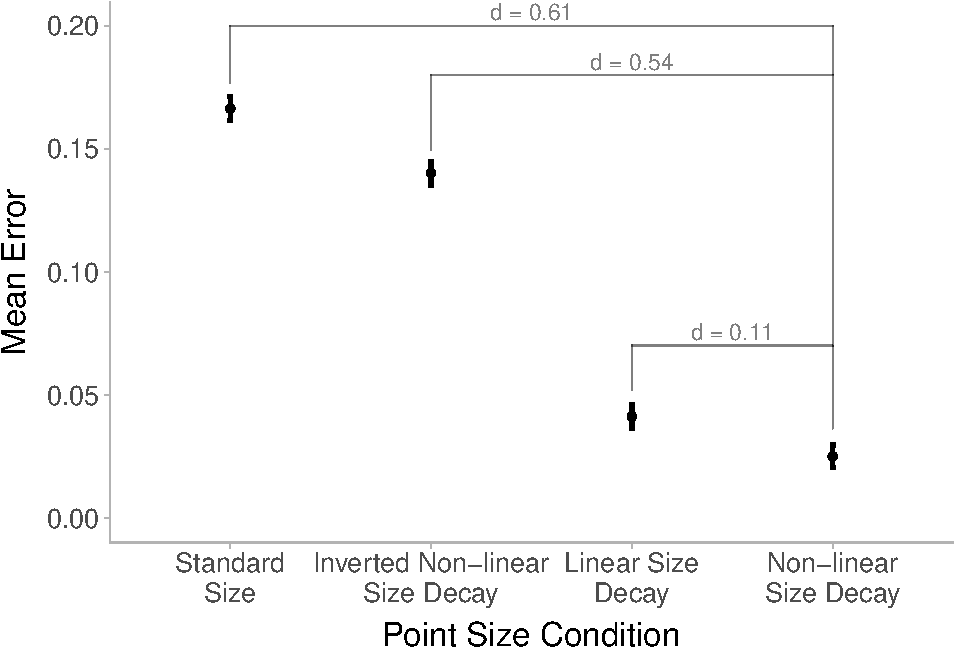
\includegraphics[width=1\linewidth]{size_and_scatterplots_files/figure-latex/dot-plot-1} \caption{Mean error in correlation estimates across the four conditions, with 95\% confidence intervals. Effect sizes between standard size and other conditions in Cohen's d are also displayed.}\label{fig:dot-plot}
\end{figure}

\begin{table}

\caption{\label{tab:contrasts-table}Contrasts between the four levels of the size decay condition.}
\centering
\resizebox{\linewidth}{!}{
\begin{tabular}[t]{lrl}
\toprule
Contrast & Z.ratio & p.value\\
\midrule
Non-linear Decay: Linear Decay & -3.99 & <0.001\\
Non-linear Decay : Inverted Non-linear Decay & -20.57 & <0.001\\
Non-linear Decay : Standard Size & -15.41 & <0.001\\
Linear Decay : Inverted Non-linear Decay & -16.86 & <0.001\\
Linear Decay : Standard Size & -11.96 & <0.001\\
\addlinespace
Inverted Non-linear Decay : Standard Size & -3.63 & 0.002\\
\bottomrule
\end{tabular}}
\end{table}

\begin{figure*}
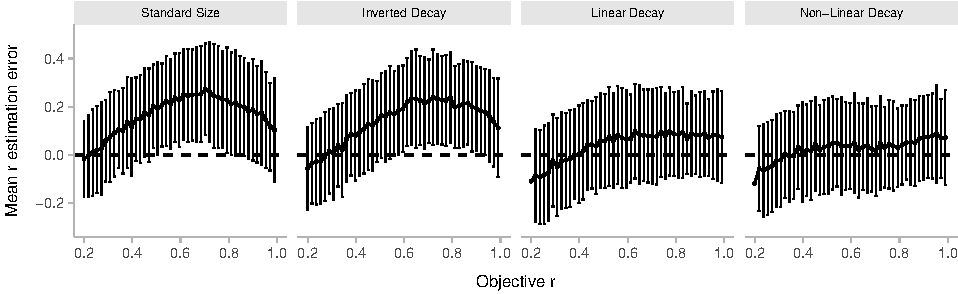
\includegraphics[width=1\linewidth]{size_and_scatterplots_files/figure-latex/changes-with-r-size-1} \caption{Participants' mean errors in \textit{r} estimates plotted against the objective \textit{r} value separately for each size decay condition. The dotted horizontal line represents accurate estimation.}\label{fig:changes-with-r-size}
\end{figure*}

All analyses were conducted using R (version 4.3.0 \cite{r_core}). Linear mixed effects models were
built using the \textbf{buildmer} (version 2.8 \cite{voeten_buildmer}) and \textbf{lme4}
(version 1.1-32 \cite{bates_lme4_2015}) packages, with size decay condition being set
as the predictor for participants' errors in correlation estimates.

Mean errors in correlation estimates for the four size decay conditions
can be seen in Figure \ref{fig:dot-plot}. A likelihood ratio test revealed that the
model including size decay condition as a predictor explained significantly more
variance than a null model (\(\chi^2\)(3) = 205.35,
\emph{p} \textless{} .001). This model has random intercepts for
items and participants. The effect here is driven by participants' errors being lower
for scatterplots with the non-linear size decay manipulation than for all other conditions,
for error being lower for scatterplots with linear size decay than for plots with
inverted non-linear decay or standard size, and for errors being higher for scatterplots
with standard size than for plots with inverted non-linear decay.

Testing for contrasts between the four levels of the size decay condition
was performed with the \textbf{emmeans} package (version 1.8.5 \cite{emmeans}), and
are shown in Table \ref{tab:contrasts-table}. The \textbf{EMAtools} (version
0.1.4 \cite{ematools}) package was used to calculate effects sizes in Cohen's d, the results of which can be seen in Figure \ref{fig:dot-plot}. The largest effect size we found was 0.61 when comparing
the non-linear size decay and standard size decay conditions. This is significantly higher
than any of the effects sizes we found in our previous work.

In addition, we find no significant difference between the experimental model
and another including graph literacy as a fixed effect (\(\chi^2\)(1) = 0.45, \emph{p} = .502), suggesting the effect we found was not driven by differences in graph literacy.

Figure \ref{fig:changes-with-r-size} shows how participants' mean errors in correlation
estimates change with the objective \emph{r} value, plotted separately for each
size decay condition. Note the close-to-zero average errors present in the non-linear size
decay condition.

We employed a method for obtaining
a measurement of dot pitch from each participant. While \autoref{visual-threshold-testing}
provides evidence that participants had no problems perceiving all the points
shown on the scatterplots, there may be some other facet of using a larger or smaller
monitor with a higher or lower resolution that could have affected the estimates
participants gave. To check this, we built a model including the dot pitch
measurement as a fixed effect. Comparing this to the experimental model revealed
a significant effect of dot pitch (\(\chi^2\)(1) = 4.44, \emph{p} = .035). There was no
interaction between size decay condition and dot pitch, with a decrease in dot
pitch of 0.1 resulting in a decrease in estimated correlation of .03.
While statistically significant, we do not consider this effect substantial
enough to warrant further discussion.

\hypertarget{discussion}{%
\section{Discussion}\label{discussion}}

As can be seen in Figure \ref{fig:changes-with-r-size},
participants' errors in correlation estimates were significantly lower when
they were presented with the non-linear size decay condition (see Figure \ref{fig:examples})
compared to when they were presented with all other conditions, providing support for our
first hypothesis. We found no support for our second hypothesis, that participants'
estimates would be least accurate in the inverted non-linear size decay condition.
Errors in this condition were indeed significantly higher than for the other two
size decay conditions, but were significantly lower than
the error with the standard size condition.

\hypertarget{increased-correlation-estimation-accuracy}{%
\subsection{Increased Correlation Estimation Accuracy}\label{increased-correlation-estimation-accuracy}}

The mean error in correlation estimation for the non-linear size decay condition used
in the present study was .025, while the equivalent condition in the second experiment
of our previous study, which used the same equations applied to contrast, resulted
in a mean error of .086 \cite{strain_2023}. Taken together, this is evidence that point
size is a much stronger channel for the manipulation of perceived correlation in
scatterplots than point contrast. If the effects we have found here and in our
previous work are being driven by increased uncertainty in the outer regions of the plots,
that we have found a large effect of point size manipulations is congruent
with research showing clear influences of stimulus size on perception and uncertainty
\cite{hong_2021, grice_1983, alais_2004}. Contrary to this, the literature linking
lower contrast to perceptual uncertainty is sparse. We interpret our results
as being supportive of the notion that correlation perception is driven
by the perception of the width of a probability distribution; our lower salience
and higher uncertainty exterior points have successfully reduced the perceived width
of this probability distribution, which has resulted in more accurate estimates
of correlation.

The lack of support for our second hypothesis was surprising, although it should
be noted that the difference between the inverted non-linear condition and the standard size
condition was small (see Figure \ref{fig:dot-plot}). The shape of the errors
in correlation estimates (see Figure \ref{fig:changes-with-r-size}) is also
very similar to that of the standard size decay condition. Despite the size channel
being more powerful than contrast with regards to correcting
for the underestimation of correlation, our results suggest it is weaker at
producing the opposing effect. In our previous work we suggested that contrast
manipulations could be used to correct for the \emph{overestimation} of the correlation
of negatively correlated scatterplots; we would not suggest the use of the size
channel for this given the results here.

\hypertarget{precision-in-correlation-estimation-is-constant}{%
\subsection{Precision in Correlation Estimation is Constant}\label{precision-in-correlation-estimation-is-constant}}

Unlike our previous work, in which the standard deviations of errors for most
conditions became smaller as the objective \emph{r} value increased, participants'
distributions of standard deviations of correlation estimates remained mostly constant. This
is unexpected, as previous work, including our own, finds precision
in \emph{r} estimation to increase as the objective \emph{r} value increases. Given that we found
this in our work manipulating point contrast \cite{strain_2023}, and
its robustness in the literature, this result is surprising. We suggest that this
is due to the nature of the stimuli. At high values of \emph{r} there is a large amount
of overlap between points in the non-linear, non-linear inverted, and linear size decay conditions (see examples in the item preparation folder in the repository linked above). It may be that this
is itself producing greater uncertainty and causing an absence of the increased
precision we would expect to see at higher \emph{r} values. While the visual character
of the scatterplots in the aforementioned conditions can account for the absence
of higher precision at higher \emph{r} values, the same cannot be said for the standard size
condition. Aside from the inverted non-linear decay condition in experiment two of
our prior work \cite{strain_2023}, the finding that precision increased with \emph{r}
was robust. Its absence here is curious given that the standard size decay condition in
the present study is identical to the full contrast conditions in our previous work.
Relying on relative judgements means
the interplay between scatterplots with different visual features must be accounted
for within a particular experiment. The stimuli as \emph{r} approaches 1 in the current
study exhibit greater levels of visual variance than the stimuli in our previous work \cite{strain_2023},
which may explain the lack of increased precision here. Further testing is required
for a more concrete explanation.

Ultimately we aim to provide tools that can be used to design visualizations more suited for the task
they are intended to support. When that task is the perception of positive correlation, we would
recommend the use of the non-linear size decay condition described here over the contrast
decay conditions we have previously tested \cite{strain_2023}. We acknowledge that
for other scatterplot tasks, such as cluster separation or numerosity perception,
the use of the manipulation described here may in fact be a hindrance, and in scenarios
where the intended usage of a scatterplot includes tasks such as these, we would not
recommend it. Instead we may recommend the use of a contrast decay condition as described
in \cite{strain_2023}, which also corrects for the underestimation bias (albeit to a
lesser degree), while not impeding other tasks.

\hypertarget{training}{%
\subsection{Training}\label{training}}

Before the experiment, participants viewed plots for a minimum of
eight seconds with examples of \emph{r} = 0.2, 0.5, 0.8, and 0.95. This was to account
for any potential unfamiliarity with scatterplots present in the samples
that we recruited; this risk is inherent in recruiting from lay populations, but we
would argue is acceptable given it leads to more generalisable and broadly
applicable findings. To test whether this training had an effect on correlation estimation,
we built a model including session half as a predictor. Comparing this
to the original model revealed no significant effect (\(\chi^2\)(1)
= 1.28, \emph{p} = 0.26),
suggesting that having more recently viewed the example plots did not have an effect
on participants' estimates of correlation.

\hypertarget{limitations}{%
\subsection{Limitations}\label{limitations}}

The data we have gathered is inherently comparative.
Despite confirming a method of obtaining dot pitch, we still have no method of obtaining
head-to-monitor distances. Taken together, these aspects of our experiment prevent us
from making concrete psychophysical conclusions,
but instead allow for findings that are rigorous to different viewing contexts and
are of particular importance for the HCI and visualization design audiences. It
may be that a high level perceptual phenomenon is responsible for the effects
we have seen here; investigating this is beyond the scope of the current study and
does not negate our findings.

\hypertarget{future-work}{%
\subsection{Future Work}\label{future-work}}

At present, we have confirmed the potential for both point contrast and size
manipulations to influence participants' perceptions of correlation in scatterplots,
each to varying degrees. It is also clear that these manipulations are not necessary,
and may even be making perception worse, at very low and high values of \emph{r}. We will therefore
investigate the effect of manipulating \emph{both} point size and contrast on correlation estimation, and we will introduce a
parameter to control the strength of this family of manipulations according to the
objective \emph{r} value itself. There is also the potential for manipulations
such as the ones described here to be applied to negatively correlated scatterplots,
which suffer from an overestimation bias \cite{sher_2017}.

%% if specified like this the section will be committed in review mode
\acknowledgments{This work was supported by funding from the University of Manchester Department of Computer Science and Division of Psychology, Communication and Human Neuroscience.}

%\bibliographystyle{abbrv}
\bibliographystyle{bib_styles/abbrv-doi}
%\bibliographystyle{abbrv-doi-narrow}
%\bibliographystyle{abbrv-doi-hyperref}
%\bibliographystyle{abbrv-doi-hyperref-narrow}

\bibliography{size-and-scatterplots}
\end{document}
